% Provenance (never printed): old terminale S material on past climates (ice cores,
% pollen, ocean sediments and oxygen isotopes, glacial-interglacial cycles, the
% astronomical rhythm told, climates of deep time), read from data. Owner (Sync 0/1):
% climate archive and proxy, ice core, glacial period, interglacial and glacial cycle,
% pollen analysis, Last Glacial Maximum. Recalled: glacier, ice sheet, ice age (Book 1,
% grade 8); the first look at the ice-core records (Book 1, grade 9); isotopes
% (physics); greenhouse gases (chemistry); the time scale (Book 1, grade 7). The
% delta notation of isotopes is Book 3's: isotope curves are read here as told,
% without a definition. The orbital theory of climate belongs to a university book:
% told here only. Physical science only, in the IPCC's calibrated words.
% Figures: figdata/grade-12/ice_age_records.py (tests/grade-12/test_ice_age_records.py).
\chapter{Klimaten van het verleden lezen}\label{ch:g12:past-climates}

Op Dome~C, \qty{3233}{m} hoog op de Oost-Antarctische ijskap, is de lucht
over het jaar gemiddeld ongeveer \qty{-55}{\degreeCelsius}. Een boor die daar werkte,
stopte op een diepte van \qty{3260}{m}, ongeveer \qty{15}{m} boven het gesteente onder
het ijs. Het diepste ijs dat ze bovenbracht, bevat kleine luchtbelletjes van zo'n
\num{800000} jaar oud: een monster van de atmosfeer van lang vóór de
eerste boeren. Dit hoofdstuk
leest het klimaat van het verleden in het ijs, in de modder van meren en van de
oceaanbodem, en in de gesteenten, en vraagt wat het zegt over vandaag.
% ledger: ipev:concordia, edc3:drilling, jouzel07:edc

\begin{omfigure}
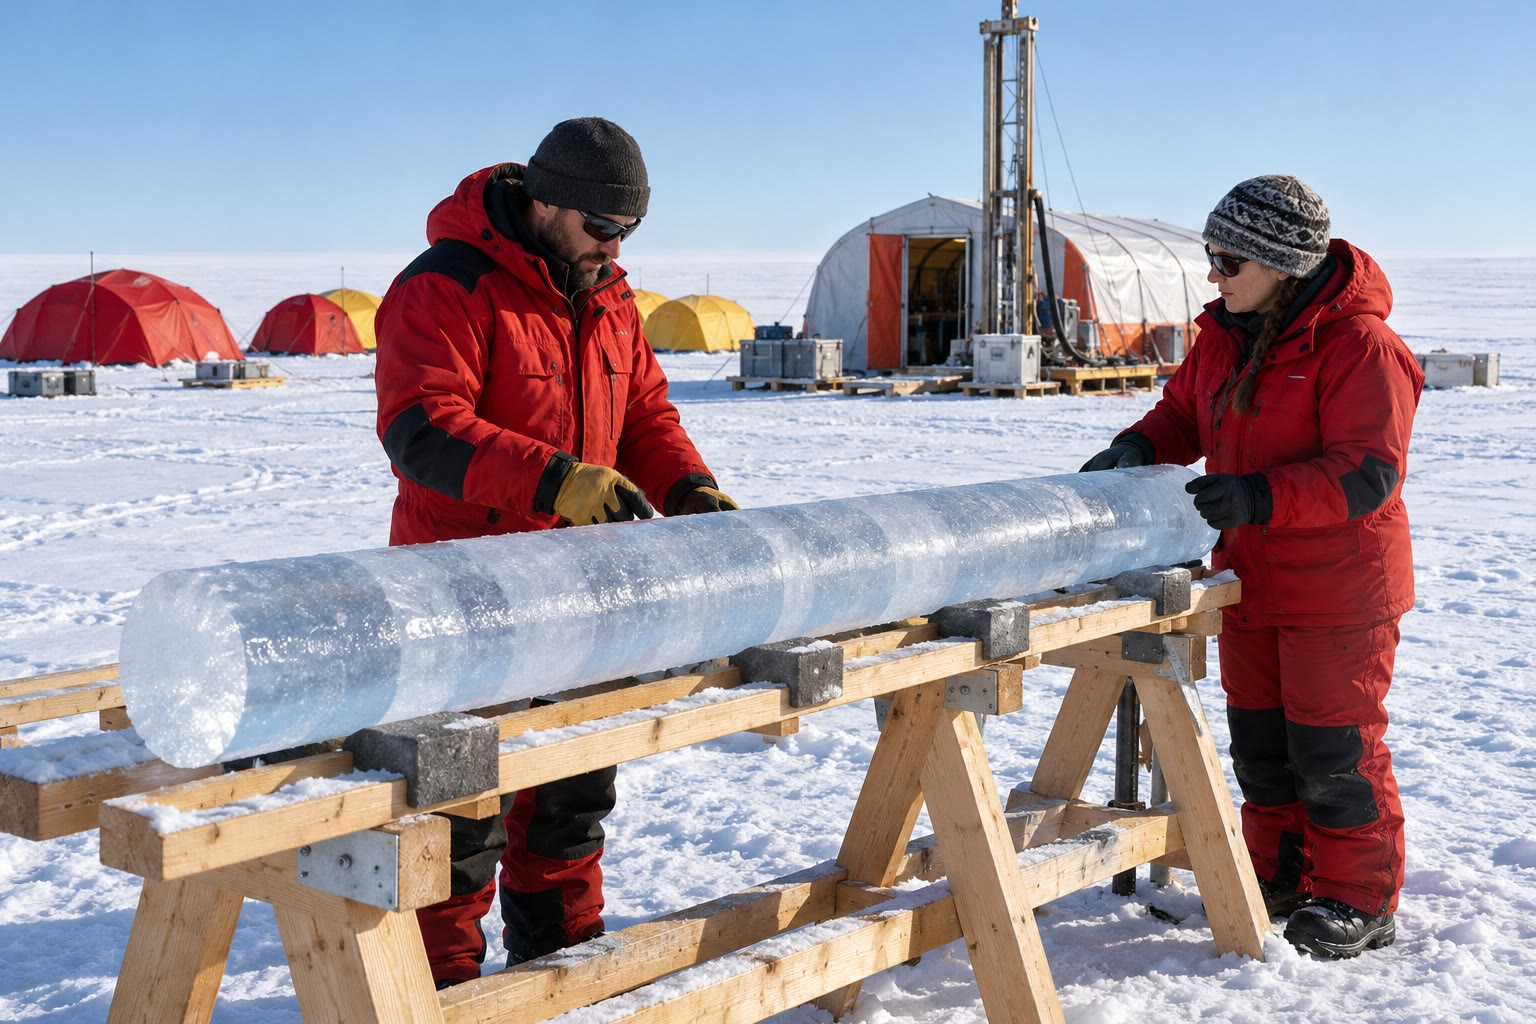
\includegraphics[width=0.56\linewidth]{images/book2/ai/g12-ice-coring-camp.jpg}

{\small Een kamp voor ijsboringen op een polaire ijskap: de boor werkt onder de
toren en de schuilplaats, en elk stuk kern wordt uitgelegd, beschreven en
ingepakt voordat het naar het laboratorium gaat. AI-illustratie.}
\end{omfigure}

\begin{recall}
Een gletsjer is een massa ijs die van jaar tot jaar blijft bestaan en onder haar
eigen gewicht stroomt; een ijskap bedekt een groot deel van een continent; een ijstijd is een
lange koude tijd waarin ijskappen zich ver buiten de polen uitbreiden (Boek 1, jaar 8).
In de \omterm{def:g12:past-climates:ice-core}{ijskernen} van Antarctica legt de sneeuw de luchttemperatuur vast en
bewaren de belletjes de lucht zelf, en de twee archieven stijgen en dalen samen
(Boek 1, jaar 9). Atomen van één element kunnen verschillen in hun aantal
neutronen: deze isotopen gedragen zich scheikundig gelijk maar verschillen in massa (de
natuurkundeboeken). Koolstofdioxide is een broeikasgas (de scheikundeboeken).
Het Kwartair begon 2.58 miljoen jaar geleden
(Boek 1, jaar 7).
\end{recall}
% ledger: ics:base.Quaternary (shared), nasaeo:o18 (snow poor in heavy isotopes)

\section{Archieven en proxy's}

Niemand mat de temperatuur van de lucht \num{20000} jaar geleden. Maar de
Aarde hield onbedoeld archieven bij: lagen ijs en modder, schelpen en
boomstammen, die elk veranderden met het klimaat waarin ze ontstonden.

\begin{definition}[Klimaatarchief; proxy]\label{def:g12:past-climates:proxy}
Een \emph{klimaatarchief}\index{klimaatarchief} is een natuurlijk materiaal dat
in lagen, de ene na de andere, is afgezet en een spoor bewaart van het klimaat van de
tijd waarin het ontstond: polair ijs, de sedimenten van meren en van de oceaanbodem, de
jaarringen van bomen, koralen, grotafzettingen. Een \emph{proxy}\index{proxy} is een
grootheid gemeten in een archief die in de plaats komt van een klimaatvariabele die
niet werd gemeten: het aandeel zware isotopen in oude sneeuw voor de luchttemperatuur,
het aandeel van elk soort pollen in meermodder voor de begroeiing
en zo voor het klimaat.
\end{definition}
% ledger: ncei:proxy, ncei:pollen, nasaeo:o18

\begin{center}
\small
\begin{tabular}{|l|l|l|}
\hline
\textbf{archief} & \textbf{\omterm{def:g12:past-climates:proxy}{proxy}} & \textbf{vertelt over} \\
\hline
polair ijs & zware isotopen van het ijs & luchttemperatuur boven het ijs \\
 & lucht in de belletjes & koolstofdioxide, methaan \\
meersedimenten, veen & pollen & begroeiing, dan klimaat \\
oceaansedimenten & zuurstofisotopen van schelpen & ijsvolume, temperatuur van diep water \\
jaarringen & ringbreedte & groeiomstandigheden, jaar na jaar \\
koralen, grotafzettingen & isotopen, groeibanden & zee- of luchttemperatuur, regen \\
\hline
\end{tabular}

\medskip
{\small De belangrijkste klimaatarchieven en enkele van hun \omterm{def:g12:past-climates:proxy}{proxy}'s.}
\end{center}
% ledger: ncei:proxy, nasaeo:o18

Elke \omterm{def:g12:past-climates:proxy}{proxy} heeft twee dingen nodig voordat hij kan worden gelezen. Hij heeft een \emph{klok} nodig:
de ouderdom van elke laag, door jaarlagen te tellen waar ze te zien zijn,
door radiometrische datering (\cref{ch:g12:age-of-the-earth}), of door het
archief te koppelen aan een ander dat al is gedateerd. En hij heeft een \emph{ijking} nodig: het
verband tussen wat wordt gemeten en de klimaatvariabele, vandaag bepaald, waar
beide samen kunnen worden gemeten.

\begin{method}[Een proxyreeks lezen]
\begin{enumerate}
  \item Zoek het archief en de \omterm{def:g12:past-climates:proxy}{proxy}: wat werd gemeten, en waarin?
  \item Zoek in welke richting de tijd op de as loopt, en in welke eenheid; controleer
        of de as van de \omterm{def:g12:past-climates:proxy}{proxy} omgekeerd is.
  \item Vertaal de \omterm{def:g12:past-climates:proxy}{proxy}: betekent een hogere waarde warmer of kouder,
        meer ijs of minder?
  \item Let op de afstand tussen de monsters: een reeks waarvan de punten
        \num{2000} jaar uit elkaar liggen, kan geen verandering tonen die een eeuw duurde.
  \item Lees de waarden af op de gevraagde data, of de gemiddelden over een tijdvak,
        en bereken veranderingen en snelheden.
  \item Zeg wat de reeks op haar plaats toont, en pas daarna of ze
        voor de hele Aarde spreekt.
\end{enumerate}
\end{method}

\section{IJskernen}

\begin{definition}[IJskern]\label{def:g12:past-climates:ice-core}
Een \emph{ijskern}\index{ijskern} is een cilinder van ijs die uit een ijskap
of een gletsjer is geboord. Zijn diepte geeft de ouderdom van het ijs, hoe dieper hoe ouder;
het ijs legt de temperatuur vast van de lucht waarin zijn sneeuw viel, en zijn
belletjes bewaren monsters van de lucht van toen.
\end{definition}
% ledger: ncei:proxy, jouzel07:edc

Verse sneeuw is grotendeels lucht. Begraven onder de sneeuw van de volgende jaren, wordt ze
samengeperst tot \emph{firn}, een samengedrukte sneeuw waarvan de poriën nog lucht doorlaten.
Bij een dichtheid van ongeveer 820 tot \qty{830}{kg/m^3}, bereikt op 50 tot \qty{120}{m}
diepte, sluiten de poriën en wordt de lucht in belletjes opgesloten. Het ijs bewaart dus twee verschillende
archieven. De lucht in de belletjes is een monster van de atmosfeer, waarvan het koolstofdioxide
en het methaan in het laboratorium worden gemeten. Het ijs zelf bewaart de
temperatuur: watermoleculen met een zware isotoop (deuterium of
zuurstof-18) condenseren gemakkelijker dan de lichte, dus hoe kouder de lucht
op weg naar de pool, hoe armer de sneeuw wordt aan zware isotopen.
% ledger: firn:close-off, nasaeo:o18

\begin{omfigure}
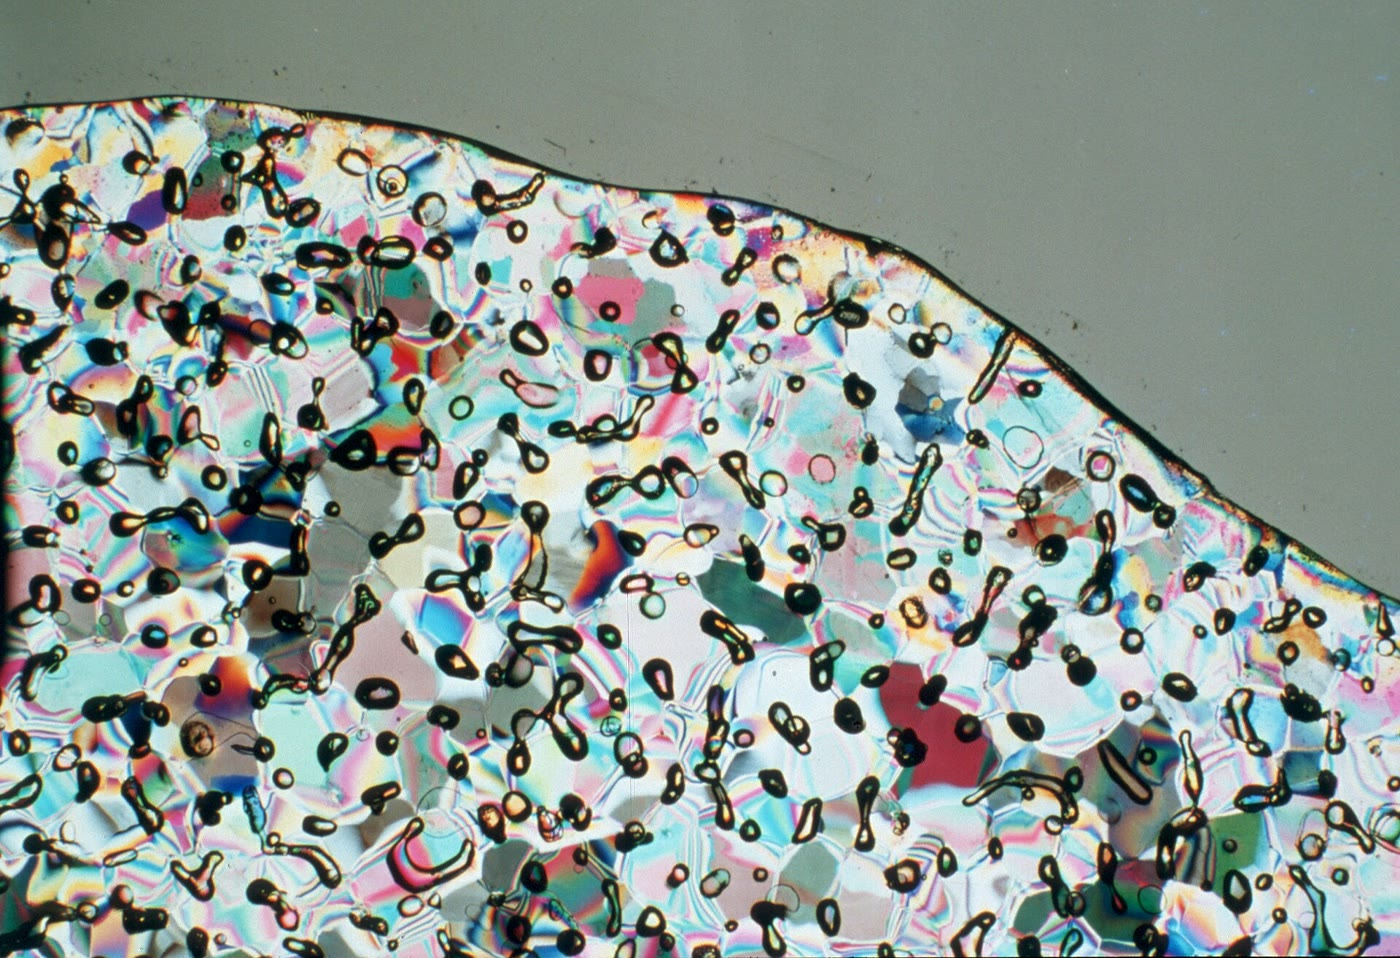
\includegraphics[width=0.50\linewidth]{images/book2/g12-ice-bubbles.jpg}

{\small Een schijfje Antarctisch ijs in gepolariseerd licht, dat de
ijskristallen kleurt: de donkere stippen zijn belletjes opgesloten lucht. Foto CSIRO
Atmospheric Research, CC~BY~3.0 (Wikimedia Commons).}
\end{omfigure}
% ledger: photo:g12-ice-bubbles

Het deuterium van de kern van Dome~C is omgezet in een temperatuur boven het
ijs, gegeven als een verandering ten opzichte van het gemiddelde van de laatste duizend jaar. Het
koolstofdioxide komt uit de belletjes van verscheidene Antarctische kernen, samengevoegd
tot één reeks. Beide staan hieronder op één tijdas.

\begin{omfigure}
\begin{tikzpicture}
\begin{axis}[omrecord, scale only axis, width=0.74\linewidth, height=4.8cm,
  xmin=0, xmax=800, x dir=reverse, ymin=-12, ymax=8, axis y line*=left,
  xtick={0,100,...,800}, ytick={-10,-5,0,5},
  xlabel={duizenden jaren vóór 1950},
  ylabel={temperatuurverandering (\unit{\degreeCelsius})}]
% data:edc-jouzel, 2-kyr means (figdata/grade-12/ice_age_records.py)
\addplot[omWarm, line width=0.7pt] table[x=age_kyr, y=temp_C] {figdata/out/grade-12-ice_age_records-edc.dat};
\end{axis}
\begin{axis}[scale only axis, width=0.74\linewidth, height=4.8cm,
  xmin=0, xmax=800, x dir=reverse, ymin=60, ymax=320, axis y line*=right,
  axis x line=none, ytick={180,220,260,300}, ylabel={koolstofdioxide (ppm)},
  every axis label/.append style={font=\small}, tick label style={font=\small}]
% data:co2-bereiter, 2-kyr means
\addplot[black, line width=0.7pt] table[x=age_kyr, y=co2_ppm] {figdata/out/grade-12-ice_age_records-co2.dat};
\coordinate (lt) at (axis cs:560,70);
\coordinate (lc) at (axis cs:560,312);
\end{axis}
\node[font=\scriptsize, text=omWarm, anchor=south] at (lt) {temperatuur op Dome~C (linkerschaal)};
\node[font=\scriptsize, anchor=north] at (lc) {koolstofdioxide (rechterschaal)};
\end{tikzpicture}

{\small Achthonderdduizend jaar Antarctisch ijs, gemiddeld over stappen van
\num{2000} jaar. Rood: de temperatuur op Dome~C ten opzichte van de laatste
duizend jaar (Jouzel en anderen, 2007); zwart: het koolstofdioxide van de
belletjes (Bereiter en anderen, 2015). Vandaag staat rechts.}
\end{omfigure}
% ledger: data:edc-jouzel, data:co2-bereiter

De twee krommen delen één patroon: een trage, grillige glijpartij naar de kou over
tienduizenden jaren, dan een snelle klim terug naar de warmte, en dan weer
de glijpartij.

\begin{definition}[Glaciaal; interglaciaal; glaciale cyclus]\label{def:g12:past-climates:glacial-cycle}
Een \emph{glaciaal}\index{glaciaal} is een koud tijdvak binnen een
ijstijd, waarin de ijskappen ver boven hun huidige omvang uitgroeien. Een
\emph{interglaciaal}\index{interglaciaal} is een warm tijdvak tussen twee
glacialen, met ijskappen ongeveer zoals vandaag of kleiner; we leven in een interglaciaal,
dat ongeveer \num{11000} jaar geleden begon. Een \emph{glaciale
cyclus}\index{glaciale cyclus} is één glaciaal met het interglaciaal dat
het afsluit.
\end{definition}
% ledger: ipcc:ref-periods (LDT ends 11 ka); the count of cycles is read from the figure (data:edc-jouzel)

Over de hele reeks loopt de temperatuur op Dome~C van
\qty{-10.6}{\degreeCelsius}, ongeveer \num{24000} jaar geleden, tot
\qty{+5.5}{\degreeCelsius}, ongeveer \num{129000} jaar geleden; het koolstofdioxide
van \qty{174}{ppm} tot \qty{299}{ppm}. De figuur, gemiddeld over \num{2000}
jaar, vlakt deze uitersten wat af. Wie de warme pieken telt, vindt acht
of negen glaciale cycli, en het sterkste ritme van de temperatuurreeks,
berekend uit haar gegevens, heeft een periode van ongeveer \num{98000} jaar.
% ledger: data:edc-jouzel, data:co2-bereiter (ice_age_records.py: edc_min_C -10.58 at 24.0 kyr, edc_max_C 5.46 at 128.7 kyr, co2 173.71 and 298.6, edc_period_kyr 97.5)

\begin{proposition}[Temperatuur en koolstofdioxide variëren samen]\label{prop:g12:past-climates:correlation}
% ledger: data:edc-jouzel, data:co2-bereiter (ice_age_records.py: r_temp_co2 0.9165, fit 266.57 + 7.827 T, 1639 pairs)
Over de laatste \num{800000} jaar varieerden de Antarctische temperatuur en het
koolstofdioxide van de lucht samen. Wie elk van de 1639 koolstofdioxidemetingen
ouder dan \num{2000} jaar koppelt aan de temperatuur op Dome~C van
dezelfde ouderdom, vindt een correlatiecoëfficiënt $r = 0.92$, en de
kleinstekwadratenlijn
\[
  \mathrm{CO_2} \approx \qty{267}{ppm} + \qty{7.8}{ppm/\degreeCelsius} \times \Delta T ,
\]
waarbij $\Delta T$ de temperatuurverandering op Dome~C is.
\end{proposition}

\begin{proof}[Hoe het wordt berekend]
Voor elk koolstofdioxidemonster wordt de temperatuur op zijn ouderdom afgelezen in de
reeks van Dome~C, door te interpoleren tussen de twee dichtstbijzijnde temperatuurpunten.
De correlatiecoëfficiënt van de 1639 paren, een getal tussen $-1$ en $1$
dat meet hoe dicht de punten bij een rechte liggen (de wiskundeboeken),
wordt samen met de kleinstekwadratenlijn berekend; beide worden berekend in het
figuurscript en gecontroleerd door de bijbehorende test.
\end{proof}

\begin{omfigure}
\begin{tikzpicture}
\begin{axis}[omrecord, width=0.70\linewidth, height=5.2cm, xmin=-12, xmax=6,
  ymin=160, ymax=310, xlabel={temperatuurverandering op Dome~C (\unit{\degreeCelsius})},
  ylabel={koolstofdioxide (ppm)}]
% data:edc-jouzel, data:co2-bereiter (pairs and fit in ice_age_records.py)
\addplot[only marks, mark=*, mark size=0.6pt, omDef, opacity=0.45] table[x=temp_C, y=co2_ppm] {figdata/out/grade-12-ice_age_records-pairs.dat};
\addplot[omThm, line width=1pt] table[x=temp_C, y=co2_ppm] {figdata/out/grade-12-ice_age_records-fit.dat};
\node[font=\scriptsize, text=omThm, anchor=south east, fill=white, inner sep=1pt] at (axis cs:-1.5,295) {kleinstekwadratenlijn, $r = 0.92$};
\end{axis}
\end{tikzpicture}

{\small Elke stip is één koolstofdioxidemeting van het Antarctische ijs,
geplaatst bij de temperatuur op Dome~C van dezelfde ouderdom: koude tijden hadden weinig koolstofdioxide,
warme tijden veel meer. Berekend uit Jouzel en anderen (2007) en
Bereiter en anderen (2015).}
\end{omfigure}

Een correlatie zegt niet wat eerst veranderde, en ook niet of een derde oorzaak
beide bewoog: de coëfficiënt zou dezelfde zijn als de temperatuur het koolstofdioxide
stuurde, als het koolstofdioxide de temperatuur stuurde, of als elk het andere aanduwde.
Wat het ritme van ongeveer \num{100000} jaar bepaalt, wordt verteld in de paragraaf over
de oceaan hieronder, en hoe koolstofdioxide op de temperatuur inwerkt, in
\cref{ch:g12:climate-change}.

\subsection{Het Laatste Glaciale Maximum}

\begin{definition}[Laatste Glaciale Maximum]\label{def:g12:past-climates:lgm}
Het \emph{Laatste Glaciale Maximum}\index{Laatste Glaciale Maximum} is de tijd, ongeveer
\num{23000} tot \num{19000} jaar geleden, waarin de ijskappen van het laatste
\omterm{def:g12:past-climates:glacial-cycle}{glaciaal} hun grootste omvang hadden.
\end{definition}
% ledger: ipcc:ref-periods

Tijdens het \omterm{def:g12:past-climates:lgm}{Laatste Glaciale Maximum} bedekten ijskappen een groot deel van Noord-Amerika en van
noordwestelijk Eurazië, en was het klimaat droger en stoffiger dan vandaag. De
evaluaties schatten dat de mondiale oppervlaktetemperatuur \qty{5}{\degreeCelsius}
tot \qty{7}{\degreeCelsius} lager was dan in 1850--1900 (\emph{gemiddelde mate van vertrouwen}),
met het koolstofdioxide op 188 tot \qty{194}{ppm}. Het water dat in de ijskappen
was opgesloten, kwam uit de oceaan: de mondiale gemiddelde zeespiegel stond 125 tot \qty{134}{m}
lager dan vandaag.
% ledger: ipcc:ref-periods, ipcc:lgm-cooling, ipcc:fig2-34, ipcc:lgm-sea, lambeck14:lgm

Een lagere zee legt de ondiepe bodem rond de continenten bloot. De kaart hieronder
verlaagt de zee met \qty{130}{m}, het midden van dat bereik, boven de bodem van
Zuidoost-Azië zoals hij vandaag is.

\begin{omfigure}
\begin{tikzpicture}
\begin{axis}[omrecord, axis equal image, width=0.62\linewidth, xmin=92, xmax=122,
  ymin=-11, ymax=24, grid=none, axis x line=box, axis y line=box,
  xtick={95,105,115}, ytick={-10,-5,...,20},
  xticklabel={\pgfmathprintnumber{\tick}\textdegree OL},
  yticklabels={10\textdegree ZB, 5\textdegree ZB, 0\textdegree, 5\textdegree NB, 10\textdegree NB, 15\textdegree NB, 20\textdegree NB}]
% data:b2-etopo-sunda (raster computed in ice_age_records.py; sea level lowered by 130 m)
\addplot graphics[xmin=91.95, xmax=122.05, ymin=-11.05, ymax=24.05] {figdata/out/grade-12-ice_age_records-sunda.png};
\node[font=\scriptsize] at (axis cs:114.5,0.5) {Borneo};
\node[font=\scriptsize, rotate=-45] at (axis cs:101.9,-1.3) {Sumatra};
\node[font=\scriptsize] at (axis cs:110.5,-8.6) {Java};
\node[font=\scriptsize, rotate=-60] at (axis cs:102.2,4.0) {Mal. Schiereil.};
\node[font=\scriptsize] at (axis cs:103,16.5) {Indochina};
\node[font=\scriptsize, align=center] at (axis cs:106.5,3.5) {Soenda-\\plat};
\node[font=\scriptsize, align=center] at (axis cs:114.5,13) {Zuid-Chinese\\Zee};
\node[font=\scriptsize, align=center] at (axis cs:96,-6) {Indische\\Oceaan};
\end{axis}
\end{tikzpicture}

{\small Zuidoost-Azië met de zee \qty{130}{m} lager dan vandaag. Groen:
land vandaag; lichtbruin: de bodem die een \qty{130}{m} lagere zeespiegel blootlegt; blauw:
zee. Het huidige reliëf wordt gebruikt, dus de kustlijn is maar bij benadering.
Berekend uit het ETOPO1-reliëf (NOAA), om de 0.1 graad.}
\end{omfigure}
% ledger: data:b2-etopo-sunda, ipcc:lgm-sea

Borneo, Sumatra en Java worden één land met het Maleisisch Schiereiland en
Indochina: het Soendaplat, vandaag onder een ondiepe zee, was droog land. Op de kaart
is een daling van maar ongeveer \qty{36}{m} genoeg om Borneo met Azië te verbinden, en Sumatra en
Java worden er nog eerder mee verbonden. Op de kaart
groeit het land boven de zee van 4.11 tot 7.16 miljoen vierkante kilometer,
1.74 keer zoveel. Over de hele Aarde verhoogt dezelfde daling van \qty{130}{m}
het aandeel van het oppervlak boven de zee van \qty{29.0}{\percent} tot
\qty{33.5}{\percent}, ongeveer 23 miljoen vierkante kilometer nieuw land.
% ledger: data:b2-etopo-sunda, data:etopo1 (ice_age_records.py: borneo_link_m -36; sunda_land_now_km2 4.105e6, lgm 7.161e6, ratio 1.744; world_land_now_frac 0.2904, lgm 0.3352, world_gain_km2 2.285e7)

\begin{example}[De laatste deglaciatie]
De opwarming die op het \omterm{def:g12:past-climates:lgm}{Laatste Glaciale Maximum} volgde, heet de laatste
deglaciale overgang; de evaluaties plaatsen haar tussen ongeveer \num{18000} en
\num{11000} jaar geleden. In de reeks van Dome~C is de gemiddelde temperatuur van het
\omterm{def:g12:past-climates:lgm}{Laatste Glaciale Maximum} (\num{23000} tot \num{19000} jaar geleden)
\qty{-9.4}{\degreeCelsius}; het gemiddelde van het volgende tijdvak, \num{11000} tot
\num{9000} jaar geleden, is \qty{-0.4}{\degreeCelsius}. De lucht boven Antarctica
warmde op met \qty{9.0}{\degreeCelsius}, terwijl haar koolstofdioxide steeg van
\qty{190}{ppm} tot \qty{264}{ppm}, met \qty{74}{ppm}. Over de hele Aarde
was de opwarming gelijk aan de geschatte afkoeling van 5 tot \qty{7}{\degreeCelsius}, ongeveer
\qty{6}{\degreeCelsius}, gespreid over de \num{7000} jaar van de overgang:
\[
  \frac{\qty{6}{\degreeCelsius}}{\num{7000}\ \text{jaar}} \approx
  \qty{0.86}{\degreeCelsius} \text{ per duizend jaar.}
\]
De zeespiegel steeg intussen van ongeveer \qty{-120}{m} tot \qty{-50}{m}, gemiddeld ongeveer
\qty{10}{mm} per jaar.
\end{example}
% ledger: ipcc:ref-periods, ipcc:lgm-cooling, ipcc:lgm-sea, data:edc-jouzel, data:co2-bereiter (ice_age_records.py: edc_lgm_C -9.389, edc_holo_C -0.360, rise 9.029; co2 189.67, 264.10, rise 74.43; ldt_mean_rate 0.857)

\begin{omfigure}
\begin{tikzpicture}
\begin{axis}[omrecord, scale only axis, width=0.74\linewidth, height=4.6cm,
  xmin=0, xmax=30, x dir=reverse, ymin=-11, ymax=12, axis y line*=left,
  xtick={0,5,...,30}, ytick={-10,-5,0},
  xlabel={duizenden jaren vóór 1950},
  ylabel={temperatuurverandering (\unit{\degreeCelsius})}]
\fill[omDef!10] (axis cs:23,-11) rectangle (axis cs:19,12);
\fill[omProp!12] (axis cs:18,-11) rectangle (axis cs:11,12);
% data:edc-jouzel, every sample
\addplot[omWarm, line width=0.6pt] table[x=age_kyr, y=temp_C] {figdata/out/grade-12-ice_age_records-edc30.dat};
\coordinate (lgm) at (axis cs:21,11.6);
\coordinate (ldt) at (axis cs:14.5,11.6);
\coordinate (lt) at (axis cs:5.5,-3.6);
\end{axis}
\begin{axis}[scale only axis, width=0.74\linewidth, height=4.6cm,
  xmin=0, xmax=30, x dir=reverse, ymin=60, ymax=290, axis y line*=right,
  axis x line=none, ytick={200,240,280}, ylabel={koolstofdioxide (ppm)},
  every axis label/.append style={font=\small}, tick label style={font=\small}]
% data:co2-bereiter, every sample
\addplot[black, line width=0.6pt, mark=*, mark size=0.5pt] table[x=age_kyr, y=co2_ppm] {figdata/out/grade-12-ice_age_records-co230.dat};
\coordinate (lc) at (axis cs:26.5,196);
\end{axis}
\node[font=\scriptsize, anchor=north, align=center] at (lgm) {Laatste Glaciale\\Maximum};
\node[font=\scriptsize, anchor=north, align=center] at (ldt) {laatste deglaciale\\overgang};
\node[font=\scriptsize, text=omWarm, anchor=north] at (lt) {temperatuur (links)};
\node[font=\scriptsize, anchor=south] at (lc) {koolstofdioxide (rechts)};
\end{tikzpicture}

{\small De laatste \num{30000} jaar op Dome~C, elke meting: de
temperatuur (rood) en het koolstofdioxide (zwart) klimmen samen uit het
\omterm{def:g12:past-climates:lgm}{Laatste Glaciale Maximum}. Gearceerd: het \omterm{def:g12:past-climates:lgm}{Laatste Glaciale Maximum} en de laatste deglaciale
overgang zoals het IPCC ze dateert. Gegevens: Jouzel en anderen (2007), Bereiter en
anderen (2015).}
\end{omfigure}
% ledger: data:edc-jouzel, data:co2-bereiter, ipcc:ref-periods

\section{Pollen}

Elke lente geven planten wolken pollen af. Het meeste gaat verloren, maar een deel
valt op meren en venen, zinkt en wordt in de modder begraven, waar het een
archief bewaart van de begroeiing die eromheen groeide. En de korrels van elke soort
plant hebben hun eigen vorm en grootte.
% ledger: ncei:pollen

\begin{omfigure}
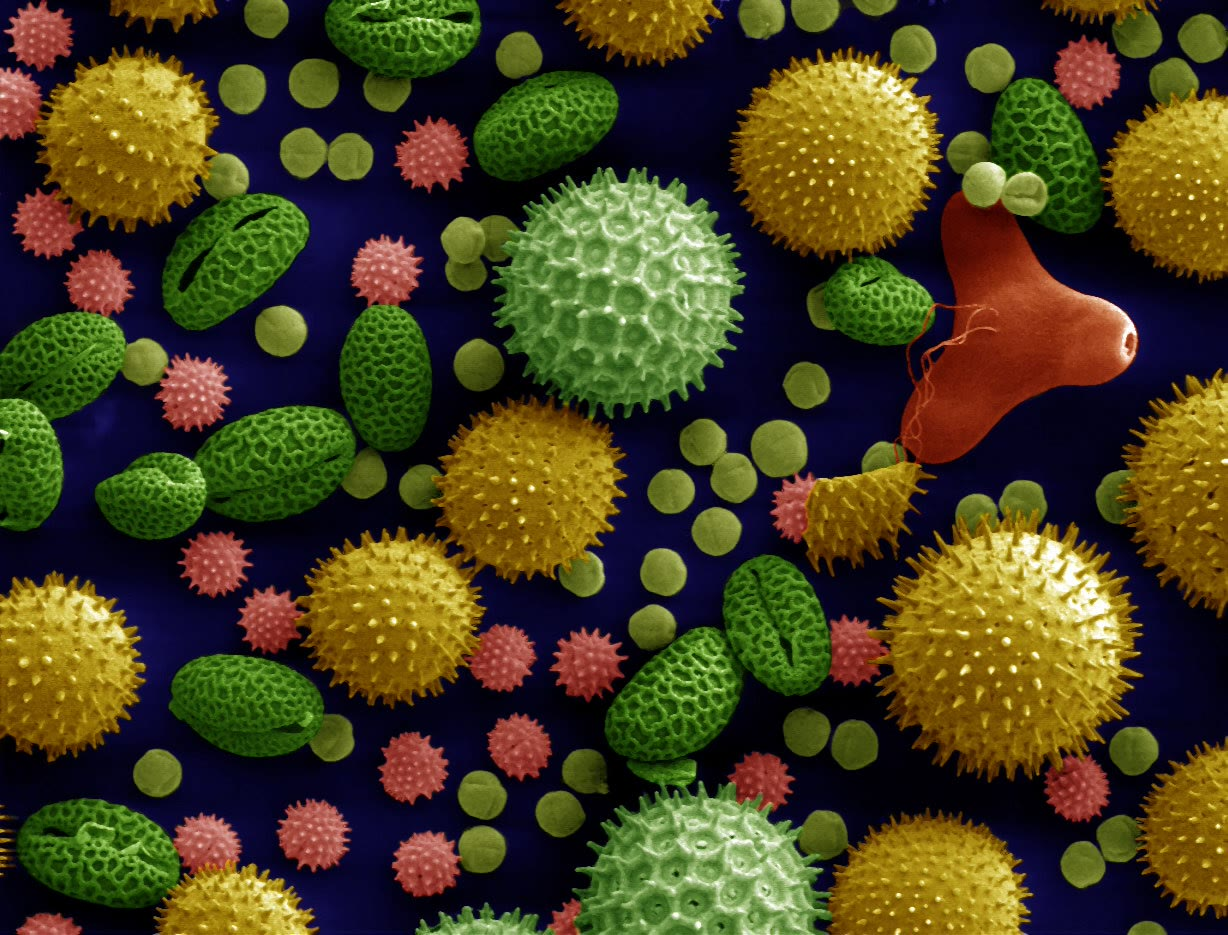
\includegraphics[width=0.46\linewidth]{images/book2/g12-pollen-sem.jpg}

{\small Pollenkorrels van vijf gewone planten (zonnebloem, haagwinde,
stokroos, lelie en sleutelbloem) gezien met een rasterelektronenmicroscoop, in
valse kleuren. Elke plantensoort heeft haar eigen vorm van korrel. Dartmouth
Electron Microscope Facility (publiek domein, via Wikimedia Commons).}
\end{omfigure}
% ledger: photo:g12-pollen

\begin{definition}[Pollenanalyse]\label{def:g12:past-climates:pollen}
\emph{Pollenanalyse}\index{pollenanalyse} is het aflezen van de vroegere
begroeiing uit het pollen dat in sedimenten bewaard is: in elke laag van een kern
worden de korrels gedetermineerd en geteld, en het aandeel van elke plantensoort,
in procent van de getelde korrels, wordt tegen de diepte uitgezet in een
\emph{pollendiagram}\index{pollendiagram}.
\end{definition}
% ledger: ncei:pollen

Het tellen van pollen op deze manier begon met de Zweedse geoloog Lennart von
Post, die in 1916 het eerste moderne \omterm{def:g12:past-climates:pollen}{pollendiagram} met getallen voorstelde;
zo'n diagram toont de diepte naar beneden op de bladzijde en één kromme voor elke
plantensoort. De begroeiing spreekt op haar beurt over het klimaat: grassen en andere
kruiden met bijna geen bomen betekenen een open, koud landschap, terwijl eik en
hazelaar warme zomers nodig hebben.
% ledger: rull18:von-post; the Varden diagram is invented (ice_age_records.py POLLEN)

\begin{omfigure}
\begin{tikzpicture}
\pgfplotsset{pollen/.style={scale only axis, height=6cm, ymin=300, ymax=600,
  y dir=reverse, xmin=0, axis x line*=bottom, axis y line*=left, axis line style={-},
  tick label style={font=\scriptsize}, title style={font=\small, yshift=-4pt, text depth=0.25ex, text height=1.6ex},
  ytick={300,350,...,600}, xmajorgrids, ymajorgrids,
  grid style={gray!22, line width=0.3pt}}}
\begin{axis}[pollen, name=p1, width=3.0cm, xmax=100, xtick={0,20,...,80}, title={kruiden},
  ylabel={diepte (cm)}, every axis label/.append style={font=\small}]
\addplot[fill=omLithSand, draw=black!70, line width=0.4pt] table[x=pct, y=depth_cm] {figdata/out/grade-12-ice_age_records-pol-herbs.dat};
\coordinate (z1) at (axis cs:0,550);
\coordinate (z2) at (axis cs:0,470);
\coordinate (z3) at (axis cs:0,425);
\end{axis}
\begin{axis}[pollen, name=p2, at={(p1.south east)}, anchor=south west, xshift=0.3cm,
  width=1.8cm, xmax=60, xtick={0,20,40}, title={berk}, yticklabels={}]
\addplot[fill=omHypsLandB, draw=black!70, line width=0.4pt] table[x=pct, y=depth_cm] {figdata/out/grade-12-ice_age_records-pol-birch.dat};
\end{axis}
\begin{axis}[pollen, name=p3, at={(p2.south east)}, anchor=south west, xshift=0.3cm,
  width=1.8cm, xmax=60, xtick={0,20,40}, title={den}, yticklabels={}]
\addplot[fill=omHypsLandA, draw=black!70, line width=0.4pt] table[x=pct, y=depth_cm] {figdata/out/grade-12-ice_age_records-pol-pine.dat};
\end{axis}
\begin{axis}[pollen, name=p4, at={(p3.south east)}, anchor=south west, xshift=0.3cm,
  width=1.2cm, xmax=40, xtick={0,20}, title={hazelaar}, yticklabels={}]
\addplot[fill=omHypsLandD, draw=black!70, line width=0.4pt] table[x=pct, y=depth_cm] {figdata/out/grade-12-ice_age_records-pol-hazel.dat};
\end{axis}
\begin{axis}[pollen, name=p5, at={(p4.south east)}, anchor=south west, xshift=0.3cm,
  width=1.5cm, xmax=50, xtick={0,20,40}, title={eik}, yticklabels={}]
\addplot[fill=omHypsLandE, draw=black!70, line width=0.4pt] table[x=pct, y=depth_cm] {figdata/out/grade-12-ice_age_records-pol-oak.dat};
\coordinate (e1) at (axis cs:50,550);
\coordinate (e2) at (axis cs:50,470);
\coordinate (e3) at (axis cs:50,425);
\coordinate (top) at (axis cs:50,300);
\coordinate (bot) at (axis cs:50,600);
\end{axis}
\draw[densely dashed, black!70] (z1) -- (e1 -| p5.east);
\draw[densely dashed, black!70] (z2) -- (e2 -| p5.east);
\draw[densely dashed, black!70] (z3) -- (e3 -| p5.east);
\node[font=\scriptsize, anchor=west] at ($(bot -| p5.east)!0.5!(e1 -| p5.east)$) {zone 1};
\node[font=\scriptsize, anchor=west] at ($(e1 -| p5.east)!0.5!(e2 -| p5.east)$) {zone 2};
\node[font=\scriptsize, anchor=west] at ($(e2 -| p5.east)!0.5!(e3 -| p5.east)$) {zone 3};
\node[font=\scriptsize, anchor=west] at ($(e3 -| p5.east)!0.5!(top -| p5.east)$) {zone 4};
\node[font=\scriptsize, anchor=north] at ($(p1.south)!0.5!(p5.south)+(0,-0.45)$) {procent van het getelde pollen};
\end{tikzpicture}

{\small Een \omterm{def:g12:past-climates:pollen}{pollendiagram} van een meer in de Varden Hills, de verzonnen streek
van deze reeks: verzonnen oefengegevens, met de opeenvolging die in veel
meren van de koelgematigde zone wordt gevonden. De onderkant van de kern (\qty{600}{cm}) is
\num{14000} jaar oud, de getoonde bovenkant (\qty{300}{cm}) \num{6000} jaar oud,
met een constante afzettingssnelheid daartussen.}
\end{omfigure}
% invented exercise data (ice_age_records.py POLLEN); no ledger row

\begin{method}[Een pollendiagram lezen]
\begin{enumerate}
  \item Lees de verticale as: diepte, de oudste lagen onderaan;
        zet diepten om in ouderdommen met de dateringen van de kern.
  \item Zoek voor elke laag de planten met de grootste aandelen.
  \item Verdeel de kern in zones, elk met haar eigen groep overheersende
        planten; leg de grenzen waar de krommen het snelst veranderen.
  \item Benoem de begroeiing van elke zone (open kruiden, berkenbos, dennenbos,
        loofbos) en het klimaat dat ze nodig heeft.
  \item Lees de zones van onder naar boven als een geschiedenis van het landschap.
\end{enumerate}
\end{method}

In het diagram hierboven is zone 1 een landschap van kruiden, met enkele berken: het
open, koude land dat het ijs achterliet. In zone 2 breidt eerst de berk zich uit, een geharde
boom; de den volgt in zone 3; en in zone 4 nemen hazelaar en eik, die warme
zomers nodig hebben, het over. Van onder naar boven gelezen vertelt de kern het einde van het
\omterm{def:g12:past-climates:glacial-cycle}{glaciaal} en de komst van de warmte van het \omterm{def:g12:past-climates:glacial-cycle}{interglaciaal}, terwijl het
bos het land weer innam.

\section{Oceaansedimenten en het astronomische ritme}

Op de bodem van de open oceaan stapelt modder zich langzaam en zonder onderbreking op,
laag na laag, miljoenen jaren lang. Ze zit vol schelpjes van
foraminiferen: eencellige organismen waarvan de schaal, een fractie van een
millimeter groot, vaak uit calciet bestaat. Sommige zweven dicht bij het
oppervlak; andere leven op de zeebodem.
% ledger: ucmp:forams, lr04:stack (benthic), photo:g12-forams (planktic)

\begin{omfigure}
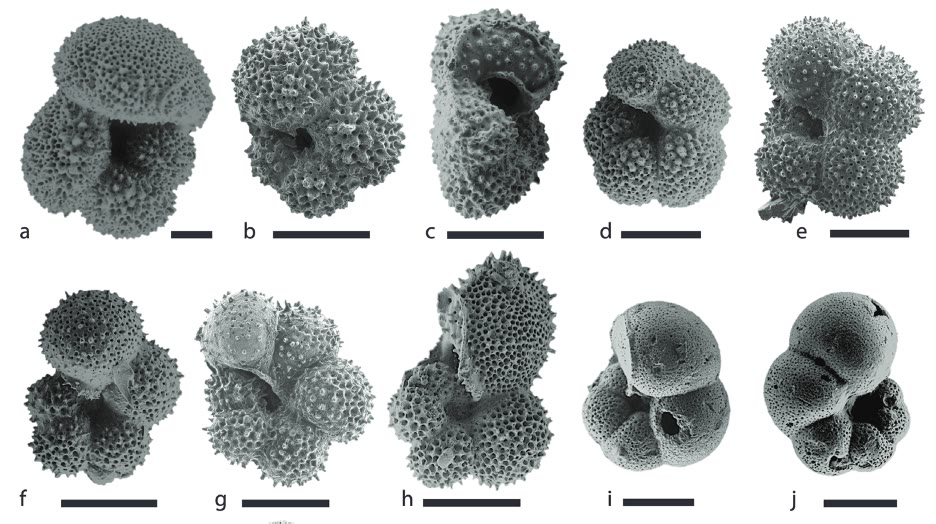
\includegraphics[width=0.62\linewidth]{images/book2/g12-planktic-foraminifera.jpg}

{\small Schelpjes van tien soorten foraminiferen die zwevend in de
oceaan leefden, gezien met een rasterelektronenmicroscoop; elke schaalstreep is
\qty{150}{\micro\metre}, dus elk schelpje is ongeveer zo groot als een zandkorrel.
Marci Robinson, USGS (publiek domein, via Wikimedia Commons).}
\end{omfigure}
% ledger: photo:g12-forams

De zuurstof van een schelp komt uit het zeewater. Water met de lichte
isotoop zuurstof-16 verdampt gemakkelijker, en de sneeuw die de ijskappen
opbouwt, is daarom arm aan zuurstof-18. Wanneer de ijskappen groeien, slaan ze
dit lichte water op, en de oceaan die achterblijft, wordt rijker aan zuurstof-18; dat
geldt ook voor de schelpen die erin groeien, en des te meer naarmate het water kouder is. Het aandeel
zuurstof-18 in de schelpen van de foraminiferen van de zeebodem, geschreven
$\delta^{18}\mathrm{O}$ en gegeven in promille, is dus een \omterm{def:g12:past-climates:proxy}{proxy} voor
het volume ijs op het land en voor de temperatuur van de \omterm{def:g10:layered-ocean:thermocline}{diepe oceaan}: hoe
hoger het is, hoe meer ijs en hoe kouder het water.
% ledger: nasaeo:o18, lr04:stack

De reeks hieronder, LR04 genoemd, stapelt de metingen van 57 kernen uit alle
oceanen tot één kromme van 5.3 miljoen jaar.

\begin{omfigure}
\begin{tikzpicture}
\begin{axis}[omrecord, scale only axis, width=0.86\linewidth, height=4.8cm,
  xmin=0, xmax=5.32, x dir=reverse, ymin=2.4, ymax=5.3, y dir=reverse,
  xtick={0,0.5,...,5}, ytick={2.5,3,...,5},
  x tick label style={/pgf/number format/.cd, fixed, precision=1},
  y tick label style={/pgf/number format/.cd, fixed, fixed zerofill, precision=1},
  xlabel={miljoenen jaren vóór 1950},
  ylabel={$\delta^{18}\mathrm{O}$ van de schelpen (\unit{\permil})}]
\fill[omProp!14] (axis cs:1.25,2.4) rectangle (axis cs:0.7,5.3);
% data:lr04 (the stack only; ice_age_records.py)
\addplot[omDef!85!black, line width=0.35pt] table[x=age_Ma, y=d18O] {figdata/out/grade-12-ice_age_records-lr04.dat};
\addplot[omThm, line width=1pt, densely dashed, unbounded coords=jump] table[x=age_Ma, y=d18O] {figdata/out/grade-12-ice_age_records-lr04mean.dat};
\coordinate (mpt) at (axis cs:0.975,2.45);
\coordinate (mm) at (axis cs:5.22,4.92);
\coordinate (arr) at (axis cs:5.12,3.9);
\end{axis}
\node[font=\scriptsize, anchor=north, align=center] at (mpt) {41 000 tot\\100 000 jaar};
\draw[omThm, line width=1pt, densely dashed] (mm) -- ($(mm)+(0.5,0)$) node[right, font=\scriptsize, text=omThm] {gemiddelden van 5.3 tot 3 en van 1 tot 0 miljoen jaar geleden};
\draw[-{Stealth}, black!70] (arr) -- ++(0,-0.9) node[midway, right, font=\scriptsize, align=left] {meer ijs,\\kouder};
\end{tikzpicture}

{\small Vijf miljoen jaar \omterm{def:g10:layered-ocean:thermocline}{diepe oceaan} in de schelpjes van foraminiferen van de zeebodem;
de verticale as is omgekeerd, zodat koude, ijsrijke tijden
laag liggen. De gestreepte lijnen zijn de gemiddelden van het eerste en het laatste deel. Gearceerd:
de overgang van een ritme van \num{41000} jaar naar een van ongeveer \num{100000}
jaar. Gegevens: Lisiecki en Raymo (2005), de LR04-stapel.}
\end{omfigure}
% ledger: data:lr04, lr04:stack, clark06:mpt

Gelezen met de methode hierboven zegt de reeks drie dingen.
\begin{itemize}
  \item \emph{De Aarde is afgekoeld en haar ijs is gegroeid.} De gemiddelde waarde
        stijgt van \qty{3.03}{\permil} tussen 5.3 en 3 miljoen jaar
        geleden tot \qty{4.15}{\permil} over het laatste miljoen jaar.
  \item \emph{De schommelingen zijn groter geworden.} Glaciale en interglaciale tijden
        wisselen elkaar over de hele reeks af, maar ze schommelen steeds wijder: tijdens
        het \omterm{def:g12:past-climates:lgm}{Laatste Glaciale Maximum} was de waarde \qty{4.92}{\permil}, tegen
        \qty{3.23}{\permil} vandaag.
  \item \emph{Het ritme is veranderd.} Tussen 2.6 en 1.3 miljoen jaar
        geleden is de sterkste periode van de reeks, berekend uit haar gegevens,
        \num{41000} jaar; over de laatste \num{700000} jaar is ze ongeveer
        \num{98000} jaar, het ritme van de \omterm{def:g12:past-climates:ice-core}{ijskernen}. De verandering vond
        plaats tussen ongeveer 1.25 en 0.7 miljoen jaar geleden.
\end{itemize}
% ledger: data:lr04, clark06:mpt (ice_age_records.py: lr04_mean_3_5Ma 3.032, lr04_mean_0_1Ma 4.147, lr04_lgm 4.92, lr04_today 3.23, periods 41.0 and 98.5 kyr)

Deze perioden zijn geen toeval. In 1976 vonden James Hays, John Imbrie en Nicholas
Shackleton in de sedimenten van de zuidelijke oceanen drie ritmes, van
\num{23000}, \num{42000} en ongeveer \num{100000} jaar, die de perioden zijn
van trage veranderingen in de baan en de as van de Aarde: de precessie van de as,
de helling van de as (ongeveer \num{41000} jaar) en de vorm van de baan
(ongeveer \num{100000} jaar). Deze veranderingen verschuiven het zonlicht dat elke
breedte in elk seizoen ontvangt, en ze bepalen het tempo van de glaciale
cycli. Hoe ze dat doen, en waarom het trage ritme van \num{100000} jaar de overhand
kreeg, is de stof van een universitaire cursus.
% ledger: hays76:periods, nasa:milankovitch, lr04:stack, clark06:mpt

\begin{dated}{2025}
In januari 2025 maakte het project Beyond EPICA bekend dat een kern die geboord is op
Little Dome~C, ongeveer \qty{35}{km} van het Concordiastation op Dome~C, in zijn bovenste
\qty{2480}{m} een ononderbroken archief bevat tot ongeveer 1.2 miljoen jaar
terug. Ze bestrijkt de tijd
waarin het glaciale ritme veranderde van \num{41000} naar \num{100000} jaar, en het
ijs en zijn lucht worden geanalyseerd.
\end{dated}
% ledger: ku25:beyond-epica, ipev25:little-dome-c

\section{Klimaten van de diepe tijd}

Verder terug dan de \omterm{def:g12:past-climates:ice-core}{ijskernen} worden de klimaten van het verleden gelezen uit
sedimenten, fossiele bladeren en bodems, en isotopen. Het IPCC heeft enkele
goed bestudeerde \emph{referentieperioden} gekozen, waarvan de klimaten helpen om
de veranderingen van vandaag en morgen te beoordelen. De grafiek hieronder geeft hun mondiale
oppervlaktetemperatuur, ten opzichte van 1850--1900.

\begin{omfigure}
\begin{tikzpicture}
\begin{axis}[omrecord, width=0.86\linewidth, height=5.4cm, xmin=-9, xmax=27,
  ymin=0.4, ymax=6.6, y dir=reverse, ytick={1,...,6}, ymajorgrids=false,
  yticklabels={{PETM, 56 Ma}, {EECO, 53--49 Ma}, {MPWP, 3.3--3.0 Ma},
    {LIG, 129--116 ka}, {LGM, 23--19 ka}, {MH, 6.5--5.5 ka}},
  y tick label style={font=\scriptsize},
  xlabel={temperatuur ten opzichte van 1850--1900 (\unit{\degreeCelsius})}]
% ipcc:fig2-34 (DEEP in ice_age_records.py)
\addplot[draw=none, mark=none, restrict expr to domain={\thisrow{tlo}}{0:30},
  error bars/.cd, x dir=both, x explicit,
  error bar style={line width=5pt, omWarm!75}, error mark=none]
  table[x expr={(\thisrow{tlo}+\thisrow{thi})/2}, y=idx,
        x error expr={(\thisrow{thi}-\thisrow{tlo})/2}] {figdata/out/grade-12-ice_age_records-deep.dat};
\addplot[draw=none, mark=none, restrict expr to domain={\thisrow{tlo}}{-30:-0.01},
  error bars/.cd, x dir=both, x explicit,
  error bar style={line width=5pt, omCold!75}, error mark=none]
  table[x expr={(\thisrow{tlo}+\thisrow{thi})/2}, y=idx,
        x error expr={(\thisrow{thi}-\thisrow{tlo})/2}] {figdata/out/grade-12-ice_age_records-deep.dat};
\draw[black!60] (axis cs:0,0.4) -- (axis cs:0,6.6);
\draw[omThm, densely dashed, line width=0.8pt] (axis cs:1.09,0.4) -- (axis cs:1.09,6.6);
\node[font=\scriptsize, text=omThm, anchor=west, fill=white, inner sep=1pt] at (axis cs:1.6,4.55) {2011--2020};
\end{axis}
\end{tikzpicture}

{\small Mondiale oppervlaktetemperatuur van zes referentieperioden uit het verleden,
zeer waarschijnlijke bereiken, ten opzichte van 1850--1900; gestreept: het decennium 2011--2020.
PETM: Paleoceen-Eoceen Thermisch Maximum; EECO: klimaatoptimum van het
Vroeg-Eoceen; MPWP: warme periode van het midden-Plioceen; LIG: laatste interglaciaal; LGM: \omterm{def:g12:past-climates:lgm}{Laatste
Glaciale Maximum}, de enige koude (blauw); MH:
midden-Holoceen. Waarden: IPCC AR6 WG1, figuur 2.34.}
\end{omfigure}
% ledger: ipcc:fig2-34, ipcc:gsat-2011-2020, ipcc:ref-periods

\begin{center}
\small
\begin{tabular}{|l|c|c|c|}
\hline
\textbf{periode} & \textbf{temperatuur (\unit{\degreeCelsius})} & \textbf{koolstofdioxide (ppm)} & \textbf{zeespiegel (m)} \\
\hline
PETM, 56 Ma & $+10$ tot $+25$ & ongeveer 900, oplopend tot 2000 & --- \\
EECO, 53--49 Ma & $+10$ tot $+18$ & 1150 tot 2500 & $+70$ tot $+76$ \\
MPWP, 3.3--3.0 Ma & $+2.5$ tot $+4.0$ & 360 tot 420 & $+5$ tot $+25$ \\
LIG, 129--116 ka & $+0.5$ tot $+1.5$ & 266 tot 282 & $+5$ tot $+10$ \\
\textcolor{omCold}{LGM, 23--19 ka} & \textcolor{omCold}{$-7$ tot $-5$} & \textcolor{omCold}{188 tot 194} & \textcolor{omCold}{$-134$ tot $-125$} \\
MH, 6.5--5.5 ka & $+0.2$ tot $+1.0$ & 260 tot 268 & $-3.5$ tot $+0.5$ \\
\hline
\end{tabular}

\medskip
{\small De referentieperioden: mondiale oppervlaktetemperatuur ten opzichte van
1850--1900, koolstofdioxide, en mondiale zeespiegel ten opzichte van 1900. IPCC
AR6 WG1, figuur 2.34.}
\end{center}
% ledger: ipcc:fig2-34

Het Paleoceen-Eoceen Thermisch Maximum was een plotse opwarming, toen een grote
puls koolstof de oceaan en de lucht bereikte: de oceaan werd zuurder
en armer aan zuurstof, en veel diepzeesoorten stierven uit. In het klimaatoptimum
van het Vroeg-Eoceen bleef het koolstofdioxide miljoenen jaren boven \qty{1000}{ppm},
er was geen polair ijs, en bossen die bijna tropisch waren, groeiden
op \ang{70} ZB. De warme periode van het midden-Plioceen is de laatste keer dat het koolstofdioxide
dicht bij dat van vandaag lag: het noordpoolgebied was veel warmer dan nu, en de zee
stond hoger. In het laatste interglaciaal waren de ijskappen van Groenland en West-Antarctica
kleiner en de zee hoger dan vandaag, en leefden er nijlpaarden
in Groot-Brittannië.
% ledger: ipcc:ref-periods, ipcc:fig2-34, ipcc:mpwp-eeco

Deze archieven plaatsen vandaag in perspectief, en het IPCC maakt de vergelijking
zelf. In 2019 was het koolstofdioxide van de lucht hoger dan op enig moment in
minstens twee miljoen jaar (\emph{hoge mate van vertrouwen}), en de stijgingen van koolstofdioxide
en methaan sinds 1750 overtreffen ver de natuurlijke veranderingen tussen glacialen
en interglacialen over minstens \num{800000} jaar (\emph{zeer hoge mate
van vertrouwen}). De mondiale oppervlaktetemperatuur is sinds 1970 sneller gestegen dan
in enige andere periode van 50 jaar over minstens de laatste \num{2000} jaar
(\emph{hoge mate van vertrouwen}). Het decennium 2011--2020 was warmer dan de warmste
eeuwen van het huidige \omterm{def:g12:past-climates:glacial-cycle}{interglaciaal}, ongeveer \num{6500} jaar geleden, en lag dicht
bij de warmte van het laatste interglaciaal, ongeveer \num{125000} jaar geleden
(\emph{gemiddelde mate van vertrouwen}).
% ledger: ipcc:co2-ch4-800kyr, ipcc:fastest-2000yr, ipcc:co2-2myr

Ook de snelheid van de verandering kan worden vergeleken. Van 1970 tot 2025 is de trend van
de mondiale temperatuurreeks \qty{0.20}{\degreeCelsius} per decennium, of
ongeveer \qty{20}{\degreeCelsius} per duizend jaar als ze zo zou aanhouden; de
opwarming uit het laatste \omterm{def:g12:past-climates:glacial-cycle}{glaciaal} bedroeg gemiddeld ongeveer
\qty{0.86}{\degreeCelsius} per duizend jaar. De oorzaken van de huidige verandering,
en wat ze kan worden, zijn het onderwerp van \cref{ch:g12:climate-change}.
% ledger: data:gistemp (ice_age_records.py: rate_1970_2025_C_per_decade 0.2012), ipcc:lgm-cooling, ipcc:ref-periods

\section{Oefeningen}

\begin{exercise}[$\star$]\label{exo:g12:past-climates:1}
Geef de term: (a) een grootheid gemeten in een archief die in de plaats komt van een
niet-gemeten klimaatvariabele; (b) een cilinder van ijs die uit een ijskap is geboord;
(c) een warm tijdvak tussen twee glacialen; (d) het aflezen van de vroegere
begroeiing uit fossiel pollen; (e) de tijd, ongeveer \num{23000} tot \num{19000}
jaar geleden, waarin de laatste ijskappen het grootst waren.
\end{exercise}

\begin{exercise}[$\star$]\label{exo:g12:past-climates:2}
Noem voor elke \omterm{def:g12:past-climates:proxy}{proxy} zijn archief en waarover hij vertelt: (a) de lucht in
belletjes; (b) het aandeel eikenpollen; (c) het zuurstof-18 van de schelpjes van
foraminiferen van de zeebodem; (d) de breedte van jaarringen.
\end{exercise}

\begin{exercise}[$\star$]\label{exo:g12:past-climates:3}
Tijdens de laatste deglaciale overgang, van ongeveer \num{18000} tot \num{11000}
jaar geleden, steeg de zeespiegel van ongeveer \qty{-120}{m} tot \qty{-50}{m}. (a) Bereken
de gemiddelde stijgsnelheid, in millimeter per jaar. (b) Van 2006 tot 2018 steeg de zeespiegel
met \qty{3.7}{mm} per jaar. Vergelijk.
\end{exercise}

\begin{exercise}[$\star$]\label{exo:g12:past-climates:4}
De mondiale temperatuur steeg met \qty{0.20}{\degreeCelsius} per decennium van
1970 tot 2025. Druk deze snelheid uit per eeuw en per duizend jaar.
\end{exercise}

\begin{exercise}[$\star$]\label{exo:g12:past-climates:5}
Hays, Imbrie en Shackleton vonden drie ritmes in oceaansedimenten:
\num{23000}, \num{42000} en ongeveer \num{100000} jaar. (a) Koppel elk aan de
precessie van de as, de helling van de as en de vorm van de baan.
(b) Hoeveel cycli van \num{41000} jaar passen er in \num{1000000} jaar? Hoeveel
cycli van \num{100000} jaar?
\end{exercise}

\begin{exercise}[$\star\star$]\label{exo:g12:past-climates:6}
De kleinstekwadratenlijn van het hoofdstuk is $\mathrm{CO_2} \approx 266.6 +
7.83\,\Delta T$ (ppm, met $\Delta T$ in \unit{\degreeCelsius}).
(a) Voorspel het koolstofdioxide voor de gemiddelde temperatuur van het \omterm{def:g12:past-climates:lgm}{Laatste Glaciale
Maximum} op Dome~C, \qty{-9.4}{\degreeCelsius}, en vergelijk met de gemeten
\qty{190}{ppm}. (b) Voorspel het voor het warmste punt, \qty{+5.5}{\degreeCelsius},
en vergelijk met de hoogste gemeten waarde, \qty{299}{ppm}. (c) Gebruik de lijn
om de temperatuur op Dome~C te schatten die bij \qty{427}{ppm} zou horen, de
waarde van 2025 op Mauna Loa. Waarom is dit laatste gebruik van de lijn niet gerechtvaardigd?
\end{exercise}

\begin{exercise}[$\star\star$]\label{exo:g12:past-climates:7}
Gebruik het \omterm{def:g12:past-climates:pollen}{pollendiagram} van het meer in de Varden Hills. (a) Wat is het overheersende
pollen op \qty{580}{cm}, en op welk landschap wijst het? (b) Dezelfde
vraag op \qty{340}{cm}. (c) Welke boom breidt zich als eerste uit na de kou, en
welke bomen komen het laatst? (d) Waarom kan de komst van een boom achterblijven bij de
opwarming die haar mogelijk maakte?
\end{exercise}

\begin{exercise}[$\star\star$]\label{exo:g12:past-climates:8}
In dezelfde kern is de modder op \qty{600}{cm} \num{14000} jaar oud en die
op \qty{300}{cm} \num{6000} jaar oud, met een constante afzettingssnelheid.
(a) Bereken deze snelheid in millimeter per jaar. (b) Bepaal de ouderdom van de grens
tussen zone 2 en 3, op \qty{470}{cm}. (c) Hoeveel jaar stelt een plakje van
\qty{1}{cm} dik voor?
\end{exercise}

\begin{exercise}[$\star\star$]\label{exo:g12:past-climates:9}
Op de kaart van Zuidoost-Azië groeit het land boven de zee van 4.11 tot
7.16 miljoen vierkante kilometer wanneer de zee met \qty{130}{m} wordt verlaagd.
(a) Bereken de winst en haar percentage. (b) Op de kaart is een daling van ongeveer
\qty{36}{m} genoeg om Borneo met Azië te verbinden. Was het eiland gedurende het hele \omterm{def:g12:past-climates:lgm}{Laatste
Glaciale Maximum} verbonden? Leg uit. (c) Waarom is de kustlijn van de kaart maar bij
benadering?
\end{exercise}

\begin{exercise}[$\star\star$]\label{exo:g12:past-climates:10}
In de reeks LR04 is de waarde tijdens het \omterm{def:g12:past-climates:lgm}{Laatste Glaciale Maximum}
\qty{4.92}{\permil} en die van vandaag \qty{3.23}{\permil}. (a) Welke is de hoogste,
en verwacht je dat? Leg uit met de ijskappen. (b) Waarom is de
verticale as van de reeks omgekeerd getekend?
\end{exercise}

\begin{exercise}[$\star\star$]\label{exo:g12:past-climates:11}
Een vriend zegt: ``De correlatie van 0.92 tussen de Antarctische temperatuur
en het koolstofdioxide bewijst dat koolstofdioxide de ijstijden stuurde.''
(a) Wat toont een correlatie, en wat toont ze niet? (b) Geef twee
andere verklaringen die dezelfde correlatie zouden geven. (c) Wat voor
informatie over de twee reeksen zou helpen om te beslissen?
\end{exercise}

\begin{exercise}[$\star\star\star$]\label{exo:g12:past-climates:12}
De sterkste periode van de reeks LR04 is \num{41000} jaar tussen 2.6
en 1.3 miljoen jaar geleden, en \num{98500} jaar over de laatste \num{700000}
jaar. (a) Hoeveel cycli bevat elk venster? (b) Welke verandering van de
baan of de as van de Aarde past bij elke periode? (c) Leg uit waarom een reeks met
één monster om de \num{2000} jaar deze ritmes kan tonen, maar geen verandering
die een eeuw duurde.
\end{exercise}

\begin{exercise}[$\star\star\star$]\label{exo:g12:past-climates:13}
De stijgsnelheid van het koolstofdioxide was 192 tot \qty{198}{ppm} per eeuw in
1995--2014. Tijdens het Paleoceen-Eoceen Thermisch Maximum was ze 4 tot
\qty{42}{ppm} per eeuw, en tijdens de laatste deglaciale overgang hoogstens
ongeveer \qty{10}{ppm} per eeuw. (a) Hoeveel keer sneller was de recente stijging
dan de snelste stijging van de laatste deglaciatie? (b) Dan de traagste en de
snelste schatting voor het PETM? (c) De stijging van het PETM ging van ongeveer 900 tot ongeveer
\qty{2000}{ppm}. Hoe lang zou ze hebben geduurd bij \qty{42}{ppm} per eeuw,
en bij de snelheid van vandaag?
\end{exercise}

\begin{exercise}[$\star\star\star$]\label{exo:g12:past-climates:14}
Het IPCC schat dat de mondiale temperatuur met 1 tot
\qty{1.5}{\degreeCelsius} per duizend jaar steeg in het snelste deel van de laatste
deglaciatie, en dat ze boven Groenland ongeveer tien keer sneller steeg in de
eeuwen van de snelste opwarming. (a) Geef de snelheid voor Groenland in
\unit{\degreeCelsius} per duizend jaar en per decennium. (b) Vergelijk ze met de
huidige mondiale snelheid van \qty{0.20}{\degreeCelsius} per decennium. (c) Waarom mag een
plaatselijke snelheid niet rechtstreeks met een mondiale worden vergeleken?
\end{exercise}

\begin{exercise}[$\star\star\star$]\label{exo:g12:past-climates:15}
De zeespiegel stond \num{11000} jaar geleden op ongeveer \qty{-50}{m}; neem aan dat hij daarna
met een constante \qty{12}{m} per duizend jaar steeg, de gemiddelde snelheid van de voornaamste
deglaciatie. (a) Wanneer passeerde hij \qty{-36}{m}, het niveau dat Borneo
op de kaart met Azië verbindt? (b) Kon iemand na dat moment van Borneo naar
het Maleisisch Schiereiland lopen? (c) Hoe lang zou de zee erover doen om de laatste
\qty{36}{m} te stijgen, als ze met dezelfde snelheid was doorgegaan?
\end{exercise}

\begin{problem}[{Weekendprobleem --- 800 000 jaar Antarctisch ijs}]
\label{pb:g12:past-climates:1}
% ledger: data:edc-jouzel, data:co2-bereiter, data:lr04, data:gistemp, ipcc:lgm-cooling, ipcc:ref-periods, hays76:periods, clark06:mpt
% values (ice_age_records.py): edc -10.58 / +5.46, co2 173.71 / 298.6, r 0.9165, fit 266.57 + 7.827 T,
% LGM -9.389 / 189.67, 11-9 ka -0.360 / 264.10, period 97.5, rate 0.2012 per decade, ratio 23.48
Het ijs van Dome~C en de lucht in zijn belletjes geven de volgende waarden. De
temperatuur is de verandering boven het ijs ten opzichte van de laatste duizend jaar.

\begin{center}
\small
\begin{tabular}{|l|c|c|}
\hline
 \textbf{tijdstip (jaar geleden)} & \textbf{temperatuurverandering (\unit{\degreeCelsius})} & \textbf{koolstofdioxide (ppm)} \\
\hline
koudste waarde, ongeveer \num{24000} & $-10.6$ & --- \\
warmste waarde, ongeveer \num{129000} & $+5.5$ & --- \\
laagste en hoogste koolstofdioxide & --- & 174 en 299 \\
gemiddelde, \num{23000} tot \num{19000} & $-9.4$ & 190 \\
gemiddelde, \num{11000} tot \num{9000} & $-0.4$ & 264 \\
\hline
\end{tabular}
\end{center}

De sterkste periode van de temperatuurreeks is ongeveer \num{98000} jaar,
en de 1639 paren waarden geven een correlatiecoëfficiënt van 0.92.

\medskip
\noindent\textbf{Deel I --- De twee reeksen lezen.}
\begin{enumerate}
  \item Welk deel van het ijs legt de temperatuur vast, en welk het
        koolstofdioxide?
  \item Bereken het volledige bereik van de temperatuurverandering op Dome~C.
  \item Bereken het volledige bereik van het koolstofdioxide.
  \item Wat zegt een correlatiecoëfficiënt van 0.92 over de twee
        reeksen?
  \item In de figuur met de tijdas in het hoofdstuk staat vandaag rechts. Waarom
        moet je controleren in welke richting de tijd loopt voordat je zo'n figuur leest?
\end{enumerate}

\medskip
\noindent\textbf{Deel II --- Glaciale en interglaciale waarden.}
\begin{enumerate}[resume]
  \item Definieer een \omterm{def:g12:past-climates:glacial-cycle}{glaciaal} en een \omterm{def:g12:past-climates:glacial-cycle}{interglaciaal}.
  \item In welk van de twee leven we, en sinds wanneer?
  \item Hoeveel cycli van \num{98000} jaar passen er in \num{800000} jaar?
  \item Welke verandering van de baan van de Aarde heeft een periode dicht bij
        \num{100000} jaar?
  \item Wat was vóór ongeveer 1.25 miljoen jaar geleden het voornaamste ritme van
        de glaciale cycli?
\end{enumerate}

\medskip
\noindent\textbf{Deel III --- De laatste deglaciatie.}
\begin{enumerate}[resume]
  \item Hoeveel steeg de temperatuur boven Dome~C tussen het \omterm{def:g12:past-climates:lgm}{Laatste
        Glaciale Maximum} en \num{11000} tot \num{9000} jaar geleden?
  \item Hoeveel steeg het koolstofdioxide over hetzelfde tijdvak?
  \item De mondiale temperatuur van het \omterm{def:g12:past-climates:lgm}{Laatste Glaciale Maximum} lag 5 tot
        \qty{7}{\degreeCelsius} onder die van 1850--1900. Neem het midden van
        dit bereik. Is de verandering in Antarctica groter of kleiner?
  \item De laatste deglaciale overgang duurde van \num{18000} tot
        \num{11000} jaar geleden. Hoe lang is dat?
  \item Bereken de gemiddelde snelheid van de mondiale opwarming over de overgang, in
        \unit{\degreeCelsius} per duizend jaar.
  \item Druk deze snelheid uit in \unit{\degreeCelsius} per decennium.
\end{enumerate}

\medskip
\noindent\textbf{Deel IV --- De snelheid van vandaag vergeleken.}
\begin{enumerate}[resume]
  \item Van 1970 tot 2025 steeg de mondiale temperatuur met
        \qty{0.20}{\degreeCelsius} per decennium. Druk deze snelheid uit per
        duizend jaar.
  \item Hoeveel keer sneller is de opwarming van vandaag dan de gemiddelde opwarming van
        de laatste deglaciatie?
  \item In het snelste deel van de deglaciatie steeg de mondiale temperatuur
        met 1 tot \qty{1.5}{\degreeCelsius} per duizend jaar. Hoeveel keer
        sneller is de snelheid van vandaag dan deze?
  \item Besluit: hoeveel keer sneller dan de opwarming uit de laatste ijstijd
        is de mondiale opwarming van vandaag?
\end{enumerate}
\end{problem}
